\chapter{Der Integralsatz von Gauß}

(Einleitung siehe Aufschrieb)

\begin{theorem}
  Für $\Omega \subseteq \mathbb{R}^n$ offen sind äquivalent:
  \begin{enumerate}
    \item Plättung:\\
      $\forall \ p \in \partial \Omega \ \exists \ W \subseteq \mathbb{R}^n$ offen mit $p \in W$ und $\Phi: W\to \Phi(W)$\\
      $C^1$-Diffeomorphismus mit:
      $$\Phi(W \cap \Omega) = \mathbb{H}^n \cap \Phi(W) \text{ wobei } \mathbb{H}^n = \mathbb{R}^{n-1} \times (-\infty, 0)$$
      \includegraphics[width=.8\textwidth]{img/IX_1_Plättung.png}
    \item Subniveau:\\
      $\forall p\in \partial \Omega \ \exists W \subset \mathbb{R}^n$ offen mit $p \in W$ und $h \in C^1(W)$ mit $Dh(q) \neq 0) \\\forall q \in W$, sodass $\Omega \cap W = \{q \in W \ | \ h(q) < 0\}$
    \item Subgraph:\\
      $\forall p \in \partial\Omega \ \exists \script{U} \subseteq \mathbb{R}^{n-1}$ offen $\exists$ offenes Intervall $I \subseteq \mathbb{R} \ \exists C^1$-Funktion $u: \script{U} \to I$, sodass nach geeigneter Umnummerierung der Koordinaten gilt:
      $$\Omega \cap (\script{U} \times I) = \{(x,y) \in \script{U} \times I \ | \ y < u(x)\}$$
  \end{enumerate}
  Die Menge $\Omega$ hat $C^1$-Rand wenn eines (und damit jedes) der drei Kriterien erfüllt ist.
\end{theorem}
\begin{proof}
  siehe Aufschrieb
\end{proof}

\newpage
\begin{lemma}
  In der Situation von Satz IX.1,3) gilt:
  \begin{align*}
    \partial \Omega \cap(\script{U}\times I) &= \{(x,y) \in \script{U} \times I \ | \ y = u(x)\}\\
    (\mathbb{R}\setminus \bar{\Omega}) \cap (\script{U}\times I) &= \{(x,y) \in \mathbb{U} \times I \ | \ y > u(x)\}
  \end{align*}
  $\implies \partial \Omega$ ist $(n-1)$-dimensionale $C^1$-Untermannigfaltigkeit des $\mathbb{R}^n$ nach dem Graphenkriterium bei Untermannigfaltigkeiten.
\end{lemma}
\begin{proof}
  siehe Aufschrieb
\end{proof}

\sidenote{Vorlesung 24}{05.02.2021}
\begin{lemma}
  $\Omega \subseteq \mathbb{R}^n$ offen mit $C^1$-Rand. Dann gibt es zu $p \in \partial\Omega$ genau einen Vektor $\nu(p)\in \mathbb{R}^n$ mit
  \begin{enumerate}
    \item $\nu(p) \perp T_p(\partial \Omega)$ und $||\nu(p)|| = 1$
    \item $p + t \nu(p) \notin \Omega$ für $t$ hinreichend klein
  \end{enumerate}
  $\nu:\partial\Omega\to\mathbb{R}^n, n \mapsto \nu(p)$ ist stetig und heißt \textbf{äußere Normale} von $\Omega$.
\end{lemma}

\begin{remark}[Erinnerung: Tangentialraum]
  $\nu \in \mathbb{R}^n$ heißt \textbf{Tangentialvektor} von $M \subseteq R^n, C^1$-Untermannigfaltigkeit in $p\in M$, falls $\gamma:(-\delta, \delta) \to M$ existiert mit $\gamma(0) = p, \gamma'(0) = \nu$\\
  $T_pM = \{$Alle Tangentualvektoren$\}$ $(n-1)$-dimensionaler Untervektorraum.
\end{remark}

\begin{definition}
  Für $\Omega \subseteq \mathbb{R}^n$ sei $C^1(\bar{\Omega})$ der Unterraum aller $f\in C^1(\Omega)$, für die $f$ und $Df$ stetige Fortsetzungen auf $\partial \Omega$ besitzen. Die \textbf{Fortsetzung} wird wieder mit $f$ bezeichnet.
\end{definition}

\begin{lemma}
  Sei $\Omega = \{(x,y) \in \script{U} \times T \ | \ y<u(x)\}$ wobei $\script{U} \subseteq \mathbb{R}^{n-1}$ offen, $I = (a,b) \subseteq \mathbb{R}$ und $u \in C^1(\script{U}, I)$. Hat $X \in C^1(\bar{\Omega, \mathbb{R}^n})$ kompakten Träger in $\script{U}\times I$, so gilt:
  $$\int\limits_{\Omega} div \ X \ d\lambda^n = \int\limits_{\partial \Omega} <X, \nu> \ d\mu$$
\end{lemma}
\begin{proof}
  siehe Aufschrieb
\end{proof}

\begin{lemma}
  Sei $W_{\lambda}, \lambda \in \Lambda$, eine offene Überdeckung der kompakten Menge $K \subseteq \mathbb{R}^n$. Dann gibt es eine \textbf{untergeordnete Teilung der Eins}, d.h. es gibt eine endliche Familie von Funktionen $\psi_j \in C_c^{\infty}(\mathbb{R}^n), j \in J$, so dass gilt:
  \begin{enumerate}
    \item $\sum\limits_{j \in J} \psi_j(p) = 1 \ \ \ \forall \ p \in K$
    \item $\forall \ j \in J \ \exists \ \lambda = \lambda(j)$ mit $spt \ \psi_j \subseteq W_{\lambda}$
  \end{enumerate}
\end{lemma}
\begin{proof}
  siehe Aufschrieb
\end{proof}

\begin{theorem}[Integralsatz von Gauß]
  $\Omega \subseteq \mathbb{R}^n$ offen, beschränkt mit $C^1$-Rand und äußere Normale $\nu:\partial\Omega\to\mathbb{R}^n$. Dann gilt für $X\in C^1(\bar{\Omega}, \mathbb{R}^n)$:
  $$\int\limits_{\Omega} div \ X \ d\lambda^n = \int\limits_{\partial\Omega} <X, \nu> \ d\mu$$
\end{theorem}
\begin{proof}
  siehe Aufschrieb
\end{proof}

\begin{remark}
  Gilt auch für Gebiete, deren Rand lokal lipschitz ist (d.h. $u$ in Satz IX.1,3) ist lipschitz (siehe Buch von H.W. Alt: Lineare Funktionalanalysis) \\
  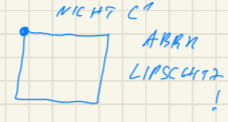
\includegraphics[width=3cm]{img/IX_7_Bem.png}
\end{remark}

\sidenote{Vorlesung 25}{08.02.2021}
\begin{example}
  Wähle $X(x) = x \implies \lambda^n(\Omega) = \frac{1}{n} \int\limits_{\Omega} div \ X \ dx = \frac{1}{n} \int\limits_{\partial \Omega} <x, \nu(x)> \ d\mu(x)$\\
  Speziell: $\alpha = \frac{\omega_{n-1}}{n}$\\
  $\Omega = B_1(0) \subseteq \mathbb{R}^n \rightarrow \nu(x) = x, \partial\Omega = S^{n-1}$ 
\end{example}

\newpage
\begin{lemma}[Greensche Formeln]
  $\Omega \subseteq \mathbb{R}^n$ offen und beschränkt mit $C^1$-Rand. Dann gilt für $u \in C^1(\bar{\Omega})$ und $v \in C^2(\bar{\Omega})$
  \begin{enumerate}
    \item $\int\limits_{\Omega}(u \triangle v + <\triangledown u, \triangledown v>) \ d\lambda^n = \int\limits_{\partial \Omega} u \frac{\partial v}{\partial \nu} \ d\mu \ \ \ (\frac{\partial v}{\partial \nu} = <\triangledown v, \nu>)$
  \end{enumerate}
  Weiter folgt für $u,v \in C^2(\bar{\Omega})$
  \begin{enumerate}[resume]
    \item $\int\limits_{\Omega} (u \triangle v - v \triangle u) \ d\lambda^n = \int\limits_{\partial \Omega}(u \frac{\partial v}{\partial \nu} - v \frac{\partial u}{\partial \nu}) \ d\mu$
  \end{enumerate}
\end{lemma}

\begin{proof}
  siehe Aufschrieb
\end{proof}

\begin{example}
  \underline{Mittelwerteigenschaft harmonischer Funktionen}\\
  Sei $\mu \in C^2(\Omega)$ eine \textbf{harmonische Funktion}, d.h. $\triangle u = 0$ in $\Omega$.\\
  Für $x_0 \in \Omega$ und $0<r<dist(x_0, \partial \Omega)$ gilt:
  $$\int\limits_{\partial B_r(x_0)} \frac{\partial u}{\partial \nu} \ d\mu \stackrel{\text{Gauß}}{=} \int\limits_{B_r(x_0)} \triangle u \ d\lambda^n = 0 \ \ \ \ \ \triangle u = div \ (\triangledown u)$$
  Auf $\mathbb{R}^n\setminus\{x_0\}$ betrachte weiter $v(x) = \gamma(||x-x_0||)$ mit $\gamma(\rho) = \begin{cases}
    \frac{\rho^{2-n}}{2-n} & , n\geq 3\\
    \log(\rho) & , n = 2
  \end{cases}$\\
  $\stackrel{\text{Ana II}}{\implies} v$ ist harmonisch auf $\mathbb{R}^n\setminus\{x_0\}$\\
  \\
  ... Rest siehe Aufschrieb
\end{example}

\begin{example}
  siehe Aufschrieb
\end{example}